\section{Auswertung}%
\label{sec:auswertung}

Ziel der Auswertung ist es einerseits das Verhältniss der Radiumisotope
$^{85}$Rd und $^{87}$Rd zu bestimmen, sowie die Landefaktoren $g_\text{F}$ und
den Kernspins $I$.
Desweiteren wird das Magnetfeld einerseits über eine statische und dynamische
Methode bestommen.
\subsection{Statische Bestimmung des Erdmagnetfeldes}%
\label{sub:statische_bestimmung_des_erdmagnetfeldes}
\begin{wrapfigure}[15]{l}{0.45\textwidth}
	\centering
	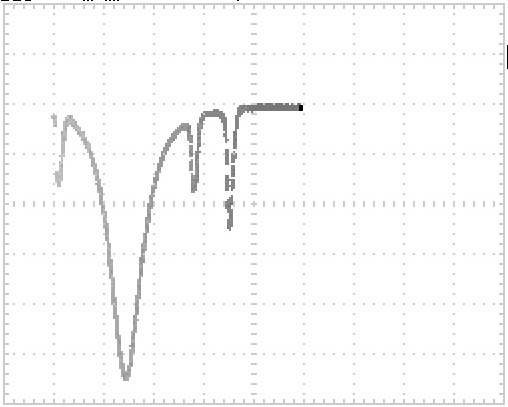
\includegraphics[width=\linewidth]{picture/Transmission_Spek_cut.JPG}
	\caption{Transmissionslinien der Rubidiumisotope $^{85}$Rb und $^{87}$Rb bei
	einer Anregungsfrequenz von \SI{100}{\kilo\hertz}.}
	\label{fig:transmission}
\end{wrapfigure}
Das Magnetfeld der Helmholtzspulen wird anhand von Formel~\ref{eq:??} 
berechnet. 
Dazu wird das Magnetfeld der Sweepspule und der horizontalen addiert. 
Durch das Wechseln der Sweepspule vom contiunus auf den statischen Betrieb
können die Resonanzstellen im Spektrum abgefahren werden.
In Abbildung~\ref{fig:transmission} ist der Fotostrom gegen die Frequenz der
RF-Spule aufgetragen. 

\subsubsection{Statische Methode}%
\label{ssub:subsubsection_name}
Der große Peak entspricht grade dem Magnetfeld welches die Horizontalkomponente
des Erdmagnetfeldes $B_\text{Erd}$ kompensiert.
Die Vertikalkomponente wird optimiert, sodass der Peak möglichst schmal ist. 
Es ergibt sich ein Magnetfeld von 
\begin{eqnarray}
	B_\text{Erd,horiz} =& \SI{36.7}{\micro\tesla}, \\
	B_\text{Erd,verti} =& \SI{19.3}{\micro\tesla}. 
\end{eqnarray}

\subsubsection{Dynamische Methode}%
\label{ssub:dynamische_methode}
Zur Bestimmung des Magnetfeldes über die Dynamische Methode, werden die
Resonanzstellen der beiden Isotope vermessen und linear gefittet.
Die angelegten magnetischen Felder $B$ sind in Abhängigkeit der Frequenz in
Tabelle~\ref{tab:b_nu} aufgeführt.
Die Magnetfelder $B$ aufgetragen gegen die Anregungsfrequenzen $\nu$ sind in
Abbildung~\ref{fig:static_B} zu sehen.

\begin{table}[h]
	\centering
	\caption{Magnetfeld zur Einstellung der Resonanz der Rubidium Isotope.}
	\label{tab:b_nu}
	\sisetup{%
		round-mode=places,
		table-format=3.1,
		round-precision=1,
	}
		\input{build/b_nu.tex}
\end{table}

Die Messwerte werden linear gefittet und der y-Achsenabschnitt $b$ spricht genau den
Offset den das Erdmangnetfeld erzeugt.
\begin{figure}[h]
	\centering
	\includegraphics[width=0.8\linewidth]{build/static_B.pdf}
	\caption{Linearer Zusammenhang der Resonanzfrequenz und dem angelegten
	magnetischen Feld für beide Isotope.}
	\label{fig:static_B}
\end{figure}
Das zur Erdmangnetfeld kompensation benötigte Feld entspricht dem Wert $b$ aus
Tabelle~\ref{tab:lin_params}.

\begin{table}[h]
	\centering
	\caption{Lineare Fitparameter zur Bestimmung des Landefaktors und des
	Erdmagnetfeldes.}
	\label{tab:lin_params}
	\sisetup{%
		round-mode=figures,
		round-precision=3,
		table-format=1.2e3
	}
	\input{build/lin_params.tex}
\end{table}



\subsection{Landefaktoren und Kernmoment der Rubidium Isotope}%
\label{sub:landefaktoren_der_rubidium_isotope}


\begin{table}[h]
	\centering
	\caption{Die Abgeleiteten größen Land\'efaktor und Kernspin aus der Steigung
	$\nu$ gegen B.}
	\label{tab:label}
	\begin{subtable}[t]{0.4\textwidth}
	\centering
	\caption{Land\'efaktoren}
	\label{tab:label}
	\input{build/lande.tex}
	\end{subtable}
	\begin{subtable}[t]{0.4\textwidth}
	\centering
	\caption{Kernspins}
	\label{tab:label}
	\input{build/kernspin.tex}
	\end{subtable}
\end{table}


\begin{table}[h]
\end{table}
\subsection{quadratischer Zeemanneffekt}%
\label{sub:quadratischer_zeemanneffekt}

B = $\SI{1}{\milli\tesla}$
\begin{equation}
	\frac{E_\text{squ} = \SI{1.04 +- 0.01e-29}{\joule}}{E_\text{lin} = 
		\SI{4.57 +- 0.02e-27}{\joule}} \approx 0.2 \%
\end{equation}



\subsection{Bestimmung des Isotopenverhaeltniss}%
\label{sub:bestimmung_des_isotopenverhaeltniss}

\subsubsection{statisch}%
\label{ssub:statisch}

\begin{equation}
	\frac{A_{85}}{A_{87}} = \frac{\SI{2.6}{\volt}}{\SI{1.4}{\volt}} = 1.86 
\end{equation}

\subsubsection{dynamisch}%
\label{ssub:dynamisch}


\begin{figure}[h]
	\centering
	\begin{subfigure}[c]{0.45\textwidth}
	\begin{center}
	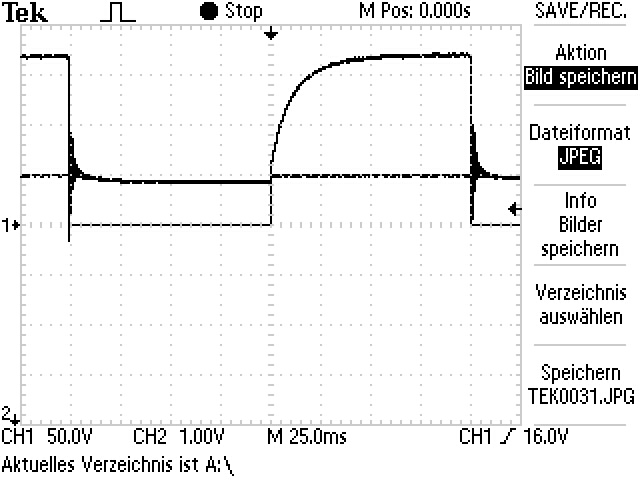
\includegraphics[width=\textwidth]{./picture/Peak_1.JPG}
	\end{center}
	\caption{Peak 1}
	\label{fig:}
	\end{subfigure}
	\begin{subfigure}[c]{0.45\textwidth}
	\begin{center}
	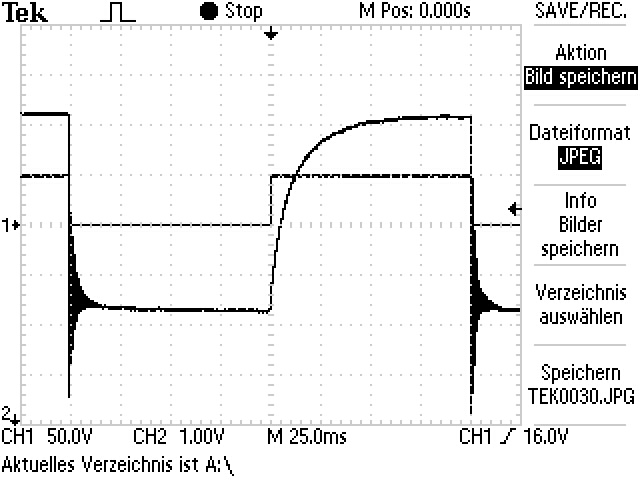
\includegraphics[width=\textwidth]{./picture/Peak_2.JPG}
	\end{center}
	\caption{Peak 2}
	\label{fig:}
	\end{subfigure}
	\caption{}
	\label{fig:}
\end{figure}

\begin{table}[h]
	\centering
	\caption{caption}
	\label{tab:label}
	\begin{subtable}[t]{0.4\textwidth}
	\centering
	\caption{caption}
		\input{build/T1.tex}
	\end{subtable}
	\begin{subtable}[t]{0.4\textwidth}
	\centering
	\caption{caption}
		\input{build/T2.tex}
	\end{subtable}
\end{table}

\begin{figure}[h]
	\centering
	\begin{subfigure}[c]{0.45\textwidth}
	\begin{center}
		\includegraphics[width=\textwidth]{build/firstPeak_9.png}
	\end{center}
	\caption{}
	\label{fig:}
	\end{subfigure}
	\begin{subfigure}[c]{0.45\textwidth}
	\begin{center}
		\includegraphics[width=\textwidth]{build/secondPeak_9.png}
	\end{center}
	\caption{}
	\label{fig:}
	\end{subfigure}

	\begin{subfigure}[c]{0.45\textwidth}
	\begin{center}
		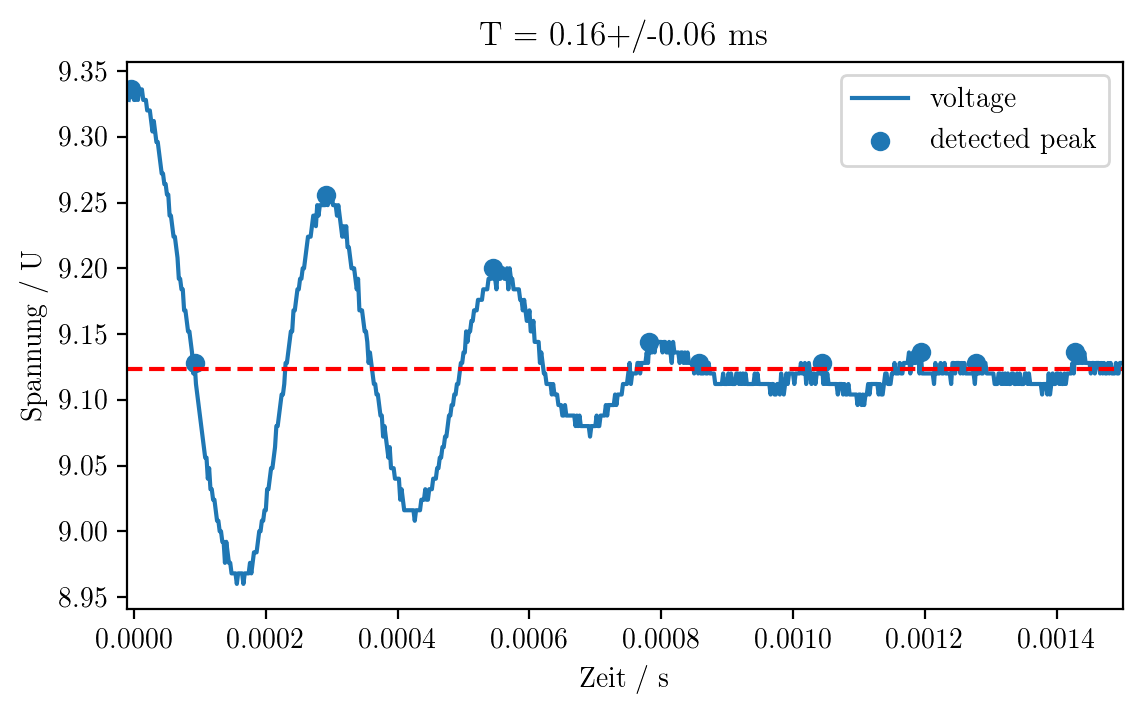
\includegraphics[width=\textwidth]{picture/firstPeak_3.png}
	\end{center}
	\caption{}
	\label{fig:}
	\end{subfigure}
	\begin{subfigure}[c]{0.45\textwidth}
	\begin{center}
		\includegraphics[width=\textwidth]{build/secondPeak_3.png}
	\end{center}
	\caption{}
	\label{fig:}
	\end{subfigure}
	\caption{}
	\label{fig:}
\end{figure}

\begin{equation}
	T(U) = a + \frac{b}{U + c}
\end{equation}

\begin{equation}
	\frac{b_{85}}{b_{87}} =
	\frac{\SI{10.7+-9.0}{\second\per\volt}}{\SI{6.6+-3.5}{\second\per\volt}} = \num{1.6 +- 1.6}
\end{equation}

\begin{figure}[h]
	\centering
	\begin{subfigure}[c]{0.45\textwidth}
	\begin{center}
		\includegraphics[width=\textwidth]{build/firstPeak.pdf}
	\end{center}
	\caption{}
	\label{fig:}
	\end{subfigure}
	\begin{subfigure}[c]{0.45\textwidth}
	\begin{center}
	\includegraphics[width=\textwidth]{build/secondPeak.pdf}
	\end{center}
	\caption{}
	\label{fig:}
	\end{subfigure}
	\caption{}
	\label{fig:}
\end{figure}


